\documentclass[a4paper,11pt]{article}
\usepackage{fullpage}
\usepackage[latin1]{inputenc}
\usepackage[T1]{fontenc}
\usepackage[normalem]{ulem}
\usepackage[english]{babel}
\usepackage{listings,babel}
\lstset{breaklines=true,basicstyle=\ttfamily}
\usepackage{graphicx}
\usepackage{moreverb}
\usepackage{url}
\usepackage{float}
\usepackage{tabularx}

\title{High Performance Dynamic Memory Controller}
\author{S\'ebastien Bourdeauducq}
\date{December 2009}
\begin{document}
\setlength{\parindent}{0pt}
\setlength{\parskip}{5pt}
\maketitle{}
\section{Specifications}
This controller is targeted at high bandwidth applications such as live video processing.

It is designed to drive 32-bit DDR SDRAM memory (which can be physically made up of two 16-bit chips).

The memory contents are accessed through a 64-bit FML (Fast Memory Link) bus with a burst length of 4. FML is a burst-oriented bus designed to ease the design of DRAM controllers. Its signaling resembles WISHBONE, but basically removes all corner cases with burst modes to save on logic resources and aspirin.

HPDMC provides high flexibility and savings on hardware by implementing a bypass mode which gives the CPU low-level access to the SDRAM command interface (address pins, bank address pins, and CKE, CS, WE, CAS and RAS). The SDRAM initialization sequence is assigned to the CPU, which should use this mode to implement it. Timing parameters are also configurable at runtime. These control interfaces are accessed on a 32-bit CSR bus, separate from the data bus. The CSR bus is a proprietary bus designed for Milkymist that helps reduce the FPGA resource usage and avoid failed timing paths on the system bus.

Due to the use of \verb!IDDR!, \verb!ODDR! and \verb!IDELAY! primitives, HPDMC currently only supports the Virtex-4 FPGAs.

\section{Architecture}

\begin{figure}[H]
\centering
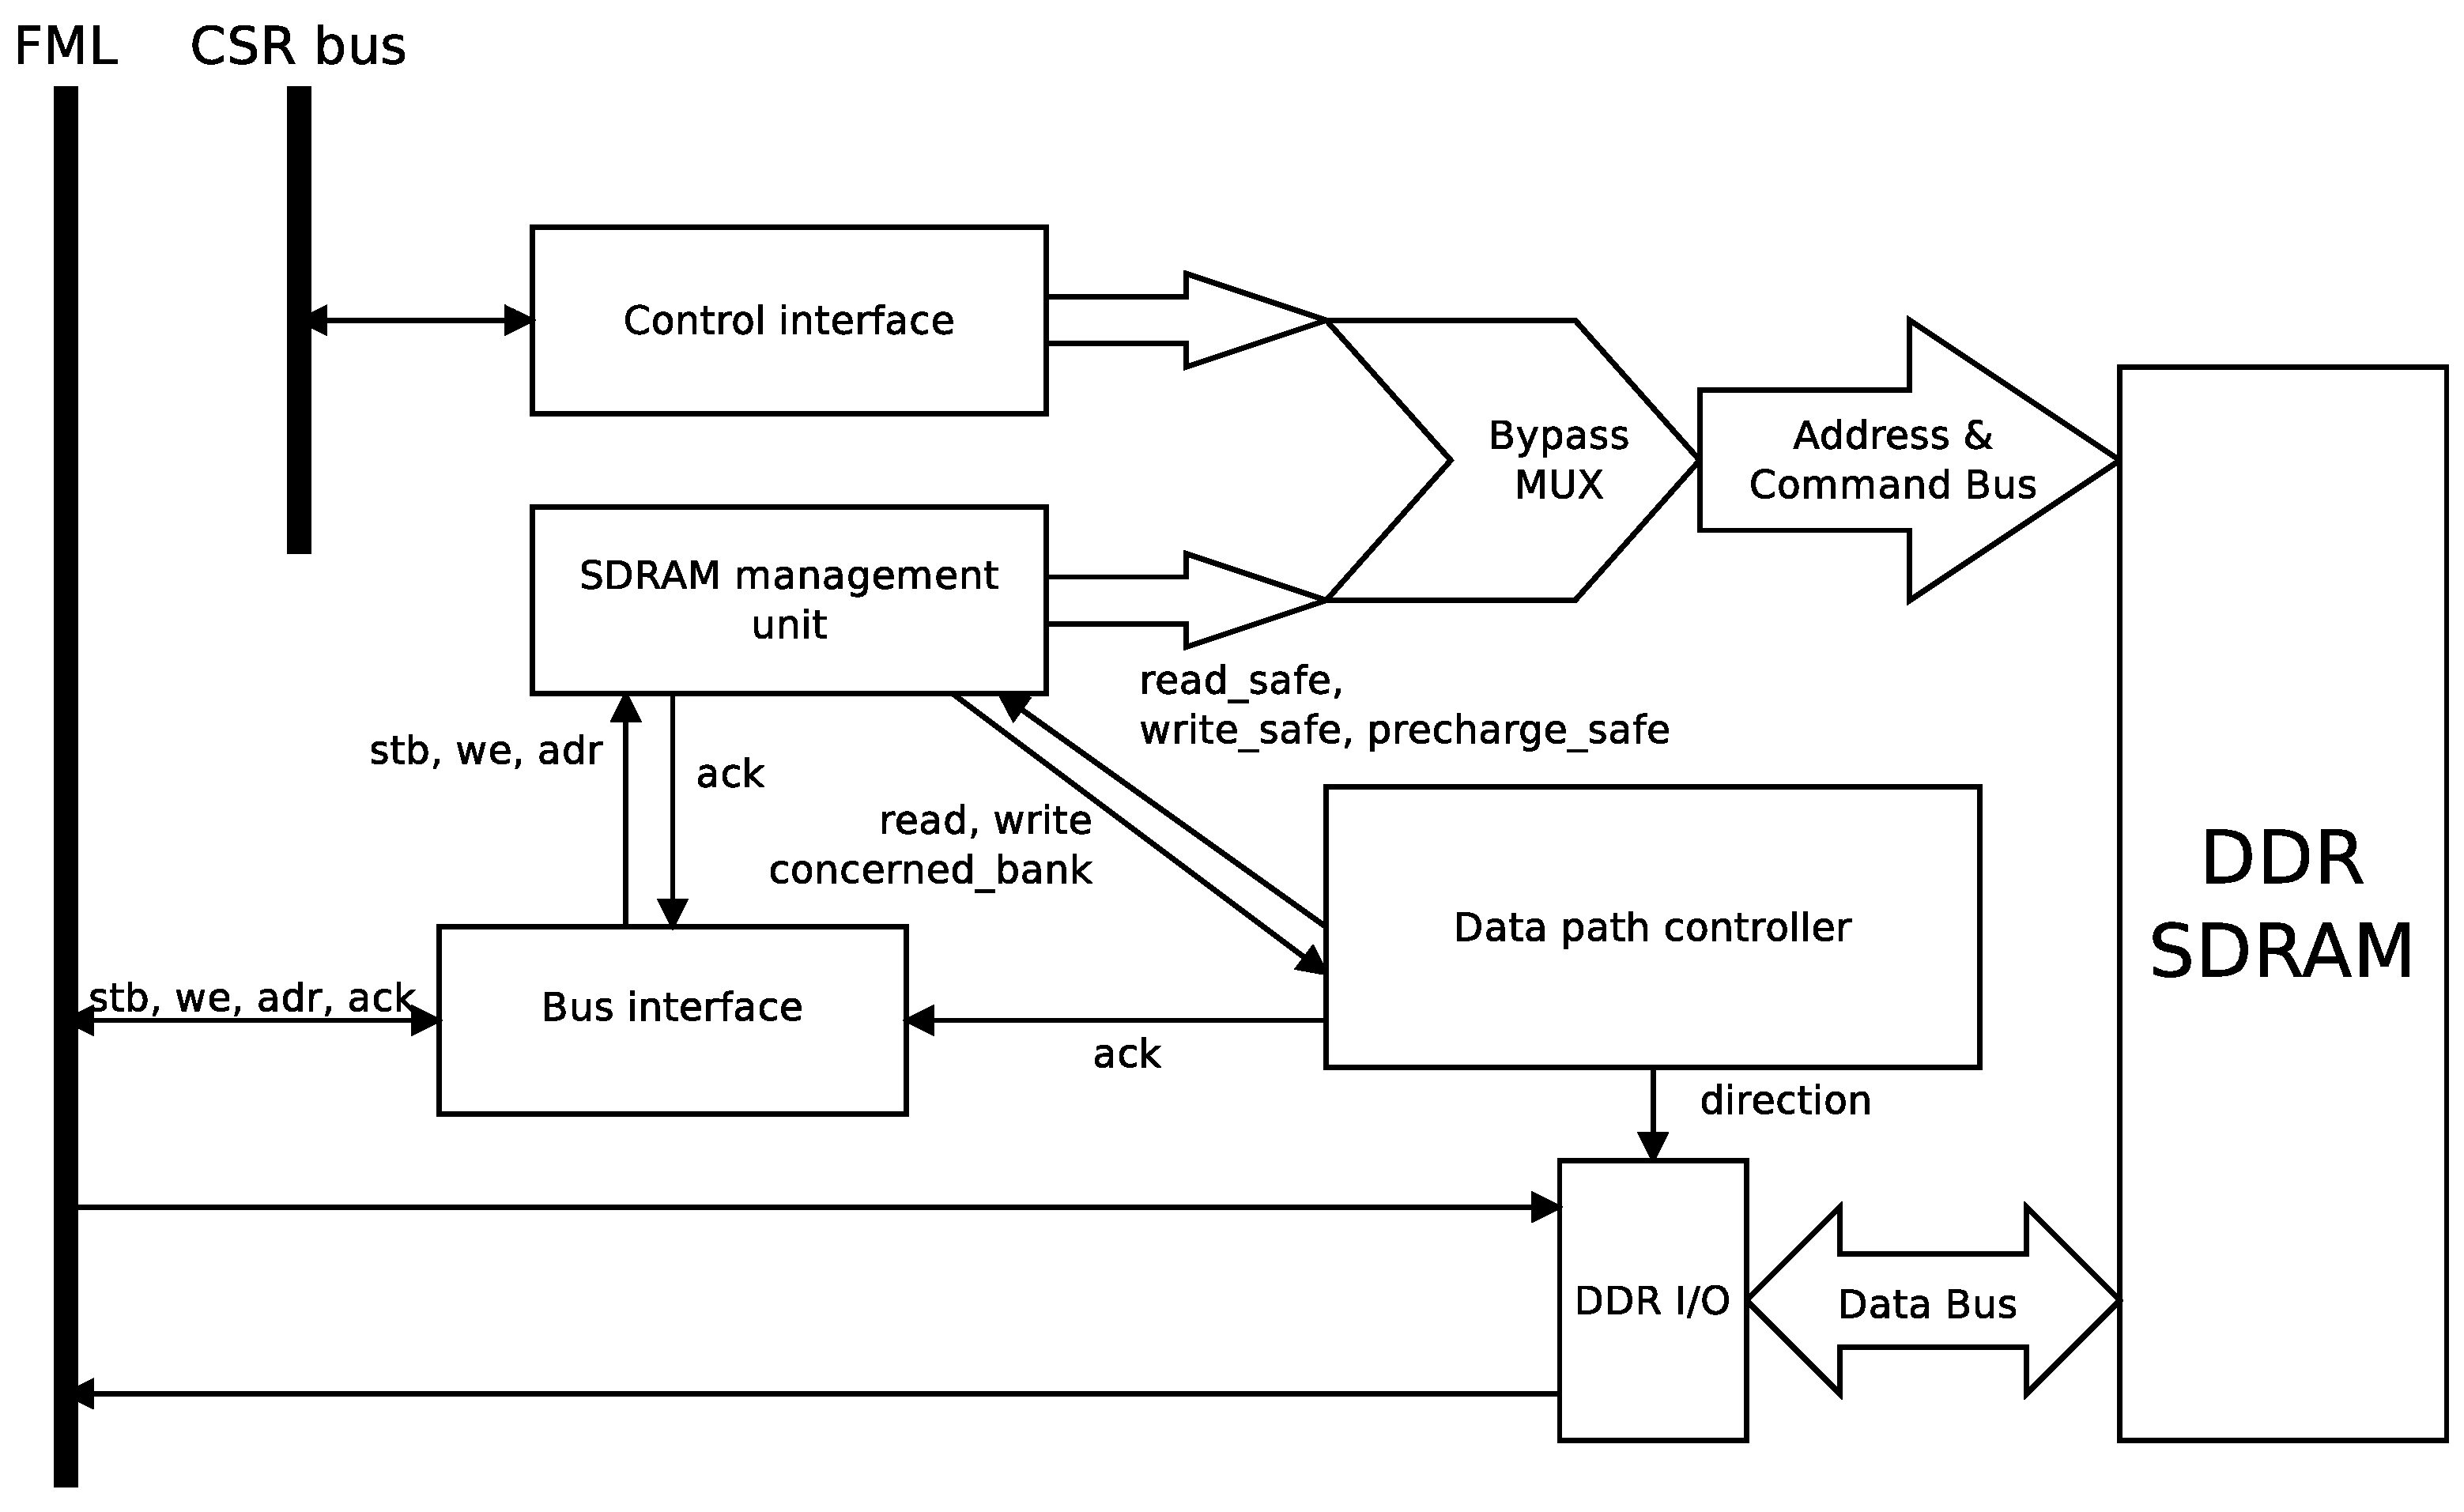
\includegraphics[height=100mm]{blockdiagram.eps}
\caption{Block diagram of the HPDMC architecture.}\label{fig:blockdiagram}
\end{figure}

\subsection{Control interface}
The control interface provides a register bank on a low-speed dedicated CSR bus, which is used to control the operating mode of the core, set timings, and initialize the SDRAM.

The interface can access directly the SDRAM address and command bus in the so-called \textit{bypass mode}. In this mode, the memory controller is disabled and the CPU can control each pin of the SDRAM control bus through the bypass register.

This mode should be used at system boot-up to perform the SDRAM initialization sequence. HPDMC does not provide a hardware state machine that does such initialization.

The mapped registers are the following (addresses are in bytes to match the addresses seen by the CPU when the CSR bus is bridged to Wishbone) :

\subsubsection{System register, offset 0x00}
\begin{tabularx}{\textwidth}{|l|l|l|X|}
\hline
\bf Bits & \bf Access & \bf Default & \bf Description \\
\hline
0 & RW & 1 & Bypass mode enable. Setting this bit transfers control of the SDRAM command and address bus from HPDMC to the system CPU. This bit should be set during the SDRAM initialization sequence and cleared during normal memory access. \\
\hline
1 & RW & 1 & Reset. This bit should be cleared during normal operation and set while reconfiguring the memory subsystem. \\
\hline
2 & RW & 0 & CKE control. This bit directly drives the CKE pin of the SDRAM and should be always set except during the first stage of the initialization sequence. The core does not support SDRAM power-down modes, so clearing this bit during normal operation results in undefined behaviour. \\
\hline
31 -- 3 & --- & 0 & Reserved. \\
\hline
\end{tabularx}

\subsubsection{Bypass register, offset 0x04}
The bypass register gives the system CPU low-level access to the SDRAM. It must be used at system power-up to initialize the SDRAM, as the controller does not provide this initialization. Such software initialization of the SDRAM provides greater flexibility and saves valuable hardware resources.

Writing once to this register issues \textbf{one} transaction to the SDRAM command bus, ie. the values written to the CS, WE, RAS and CAS bits are only taken into account for one clock cycle, and then the signals go back to their default inactive state.

The values written to this register have an effect on the SDRAM only if the controller is put in bypass mode using the system register.\\

\begin{tabularx}{\textwidth}{|l|l|l|X|}
\hline
\bf Bits & \bf Access & \bf Default & \bf Description \\
\hline
0 & W & 0 & CS control. Setting this bit activates the CS line of the SDRAM during the command transaction that results from writing to the bypass register. As the SDRAM control bus is active low, setting this bit actually puts a '0' logic level to the CS line. \\
\hline
1 & W & 0 & WE control (same as above). \\
\hline
2 & W & 0 & CAS control (same as above). \\
\hline
3 & W & 0 & RAS control (same as above). \\
\hline
16 -- 4 & RW & 0 & Address. Defines the current state of the address pins. \\
\hline
18 -- 17 & RW & 0 & Bank address. Defines the current state of the bank address pins. \\
\hline
31 -- 19 & --- & 0 & Reserved. \\
\hline
\end{tabularx}\\

\textit{NB. When this register is written, the address pins change synchronously at the same time as the command pins, so there is no need to pre-position the address bits before issuing a command. Commands like loading the mode register can therefore be performed with a single write to this register.}

\subsubsection{Timing register, offset 0x08}
This register allows the CPU to tune the behaviour of HPDMC so that it meets SDRAM timing requirements while avoiding unnecessary wait cycles.

The controller must be held in reset using the system register when the timing register is modified.\\

\begin{tabularx}{\textwidth}{|l|l|l|X|}
\hline
\bf Bits & \bf Access & \bf Default & \bf Description \\
\hline
2 -- 0 & RW & 2 & Number of clock cycles the scheduler must wait following a Precharge command. Usually referred to as $t_{RP}$ in SDRAM datasheets. \\
\hline
5 -- 3 & RW & 2 & Number of clock cycles the scheduler must wait following an Activate command. Usually referred to as $t_{RCD}$ in SDRAM datasheets. \\
\hline
6 & RW & 0 & CAS latency : 0 = CL2, 1 = CL3. CL2.5 is not supported. \\
\hline
17 -- 7 & RW & 740 & Autorefresh period, in clock cycles. This is the time between \textbf{each} Auto Refresh command that is issued to the SDRAM, not the delay between two consecutive refreshes of a particular row. Usually referred to as $t_{REFI}$ in SDRAM datasheets, which is often  7.8$\mu$s  (64ms is an improbable value for this field). \\
\hline
21 -- 18 & RW & 8 & Number of clock cycles the controller must wait following an Auto Refresh command. Usually referred to as $t_{RFC}$ in SDRAM datasheets. \\
\hline
23 -- 22 & RW & 1 & Number of clock cycles the controller must wait following the last data sent to the SDRAM during a write. Usually referred to as $t_{WR}$ in SDRAM datasheets. \\
\hline
31 -- 24 & --- & 0 & Reserved. \\
\hline
\end{tabularx}\\

\textit{NB. The default values are example only, and must be adapted to your particular setup.}

\subsubsection{Delay register, offset 0x0C}
This register controls the amount of delay that is introduced on the data lines when reading from memory. It directly controls the \verb!IDELAY! elements that are inserted between the pins and the \verb!IDDR! registers.

Writing once to the register toggles the \verb!IDELAY! control signals \textbf{once}, that is to say, the signals will be active for one clock cycle and then go back to their default zero state.

This register also controls the amount of phase shift that is introduced between the system clock and DQS (typically 90 degrees). HPDMC provides three signals, \verb!dqs_psen!, \verb!dqs_psincdec! and \verb!dqs_psdone! that should be connected to the DCM used to generate the DQS clock which is controlled by this register.

The enable and incrementation bits work the same as for \verb!IDELAY!. They should only be used when the ready bit (5) is set.\\

\begin{tabularx}{\textwidth}{|l|l|l|X|}
\hline
\bf Bits & \bf Access & \bf Default & \bf Description \\
\hline
0 & W & 0 & Resets delay to 0. If this bit is set, the others are ignored. \\
\hline
1 & W & 0 & Increments or decrements delay by one tap (typically 78ps). If the bit 2 is set at the same time this bit is written, the tap delay is incremented. Otherwise, it is decremented. \\
\hline
2 & W & 0 & Selects between incrementation and decrementation of the input tap delay. \\
\hline
3 & W & 0 & Increments or decrements the phase shift on DQS. If the bit 4 is set at the same time this bit is written, the phase shift is incremented. Otherwise, it is decremented. The phase shift is typically between -255 and 255 and is expressed in 1/256ths of the clock period. \\
\hline
4 & W & 0 & Selects between incrementation and decrementation of the DQS phase shift. \\
\hline
5 & R & 0 & When this bit is set, the DCM used to generate DQS is ready for phase shift. \\
\hline
7--6 & R & 0 & Retreives the values of the pll\_stat inputs of the core. These inputs are internally double-latched so that they can directly accept asynchronous signals. They are intended to monitor the lock status of the DCMs used to generate the SDRAM and DQS clocks. \\
\hline
31--8 & --- & 0 & Reserved. \\
\hline
\end{tabularx}

This register can be written to at any time.


\subsection{SDRAM management unit}
The SDRAM management unit is a state machine which controls sequentially the SDRAM address and command bus. Unless the core is in bypass mode, the management unit has full control over the SDRAM bus.

This unit is responsible for precharging banks, activating rows, periodically refreshing the DRAM, and sending read and write commands to the SDRAM.

It has inputs connected to the control interface registers to retreive the $t_{RP}$, $t_{RCD}$, $t_{REFI}$ and $t_{RFC}$ timing values, as well as the row idle time.

It handles read and write requests through a port made up of four elements :
\begin{itemize}
\item a strobe input
\item a write enable input (which tells if the command to send to the SDRAM should be a read or a write)
\item an address input
\item an acknowledgement output
\end{itemize}

The protocol used on these signals is close to the one employed in Wishbone. The strobe signal indicates when a new command should be completed, and remains asserted (with other signals kept constant) until the acknowledgement signal is asserted. At the next clock cycle, a new command should be presented, or the strobe signal should be de-asserted.

In HPDMC, those signals are driven by the bus interface.

The management unit also signals the data path when it has sent a read or a write command into the SDRAM. The signal is asserted exactly at the same time as the command is asserted.

It receives \verb!read_safe!, \verb!write_safe! and \verb!precharge_safe! signals from the data path, whose meanings are explained below.

\subsection{Data path controller}
The data path controller is responsible for :
\begin{itemize}
\item deciding the direction of the DQ and DQS pins
\item delaying read, write and precharge commands from the management unit that would create conflicts
\end{itemize}

The delaying of the commands is acheived through the use of three signals :
\begin{itemize}
\item \verb!read_safe! : when this signal is asserted, it is safe to send a Read command to the SDRAM. This is used to prevent conflicts on the data bus : this signal is asserted when, taking into account the CAS latency and the burst length, the resulting burst would not overlap the currently running one.
\item \verb!write_safe! : same thing, for the Write command.
\item \verb!concerned_bank[3..0]! : when the management unit issues a Read or Write command, it must inform the data path controller about the bank which the transfer takes place in, using this one-hot encoded signal.
\item \verb!precharge_safe[3..0]! : when a bit in this signal is asserted, it is safe to precharge the corresponding bank. The management unit must use this signal so as not to precharge a bank interrupting a read burst or causing a write-to-precharge violation.
\end{itemize}

The data path controller is also connected to the control interface, to retreive $t_{WR}$ and the CAS latency.

\subsection{Data path}
Data is captured from or sent to the SDRAM using \verb!IDDR! and \verb!ODDR! primitives, in order to limit timing nightmares with ISE.

When writing to the DDRAM, the \verb!ODDR! primitive puts out data synchronously to the rising and falling edges of the system clock. This was chosen to ease timing between the FML (which is clocked by the system clock) and the I/O elements without introducing additional latency cycles. The data should therefore be strobed by DQS after a short time following each system clock edge. A delay corresponding to a 90 degrees phase shift gives the best margins, and can be controlled using the delay register.

When reading from the DDRAM, the \verb!IDDR! element is also clocked by the system clock for the same reason. The data must therefore be delayed by typically one quarter of the clock cycle so that it becomes center-aligned with the system clock edges. \verb!IDELAY! primitives are used for this purpose. DQS lines are not used for reading.

\verb!ODDR!, \verb!IDDR! and \verb!IDELAY! are only supported on Virtex-4 FPGAs, but have equivalents in other families.

\subsection{Bus interface}
The bus interface is responsible for sending commands to the SDRAM management unit according to the request coming from the FML, and acknowledging bus cycles at the appropriate time.

\section{Using the core}
\subsection{Connecting}
The differential clock going to the SDRAM chips should be generated using a dedicated FPGA clocking resource, such as a DCM. It is bad practice to simply add an inverter on the negative clock line, as the inverter will also add a delay.

This DCM can also introduce a 90 degree delay on the clock and the resulting signal be used to generate DQS by connecting it to the \verb!dqs_clk! input of the HPDMC top-level.

HPDMC uses \verb!IDELAY! elements internally, but does not include the required \verb!IDELAYCTRL! primitive. You must instantiate an \verb!IDELAYCTRL! in your design, generate the 200MHz reference clock and connect it to the \verb!IDELAYCTRL! through a \verb!BUFG!. The other signals of \verb!IDELAYCTRL! can be left unused.

\subsection{Programming}
When the system is powered up, HPDMC comes up in bypass mode and the SDRAM initialization sequence should be performed from then, by controlling the pins at a low level using the bypass register.

The SDRAM must be programmed to use a fixed burst length of 8\footnote{It might seem surprising that the burst length of the SDRAM and FML are not the same. This is because DDR SDRAM counts the words on both clock edges. Here, a burst of 8 32-bit words sent at double data rate on the SDRAM side corresponds to a burst of 4 64-bit words at single data rate on the FML side.}, and a CAS latency of 2 (preferred) or 3. CAS latency 2.5 is not supported.

HPDMC's timing registers may also have to be reprogrammed to match the memory chip's parameters. If a DIMM is used, it is possible to read those parameters from the serial presence detect (SPD) EEPROM and program HPDMC accordingly.

Once the SDRAM is initialized and the timing registers are programmed, the controller can be brought up by clearing the bypass and reset bits from the system register.

You may also need to tune the data capture delay. Reset the tap count to 0 by writing bit 0 to the delay register, then increment the delay to the desired value by repeatedly writing bits 1 and 2 simultaneously.

The DQS phase shift may also be adjusted. The procedure is the same, except that the delay cannot be reset and that the ready bit should be set when writing the enable and incrementation bits. The memory is now ready to be accessed over the FML interface.

\section*{Copyright notice}
Copyright \copyright 2007-2009 S\'ebastien Bourdeauducq. \\
Permission is granted to copy, distribute and/or modify this document under the terms of the GNU Free Documentation License, Version 1.3; with no Invariant Sections, no Front-Cover Texts, and no Back-Cover Texts. A copy of the license is included in the LICENSE.FDL file at the root of the Milkymist source distribution.

\end{document}
